
\section{DHCP}

\subsection{Скриншоты}

\begin{center}

    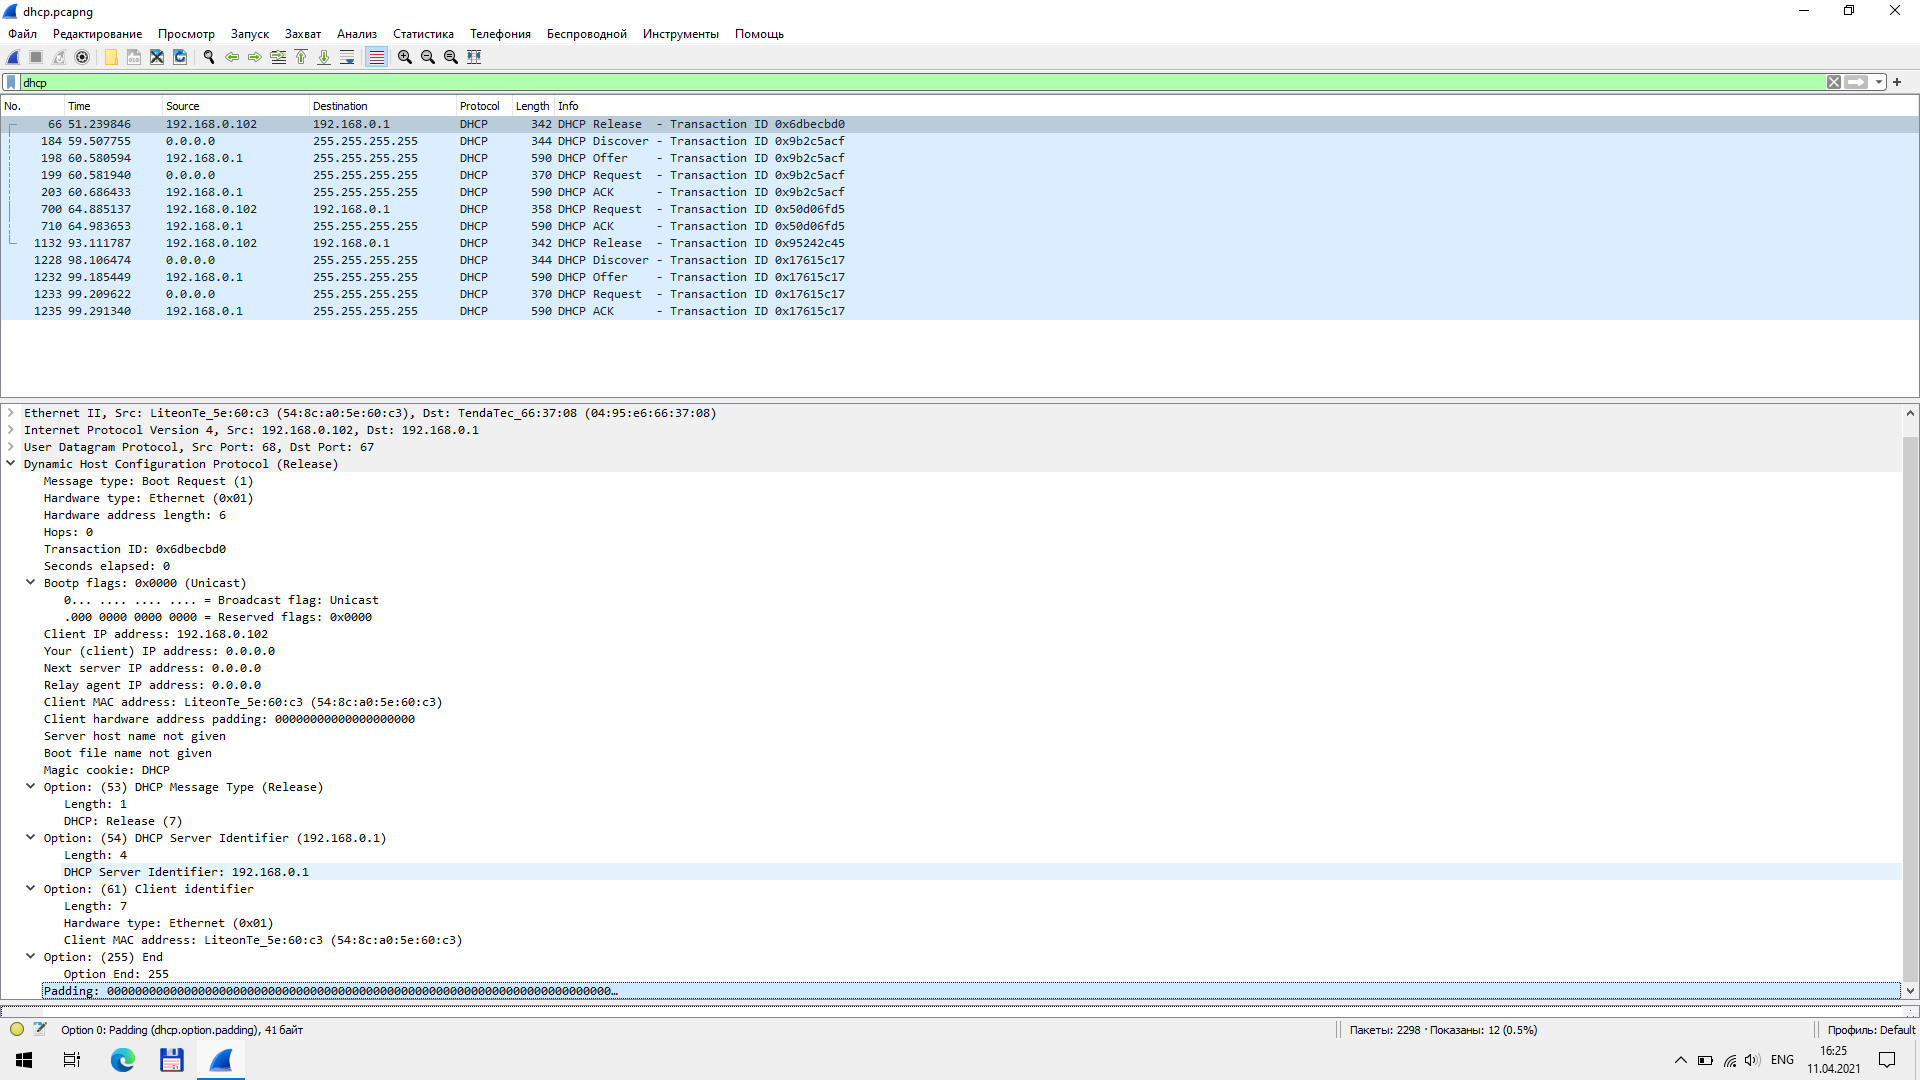
\includegraphics[width=\textwidth]{screenshots/dhcp_release_1}

    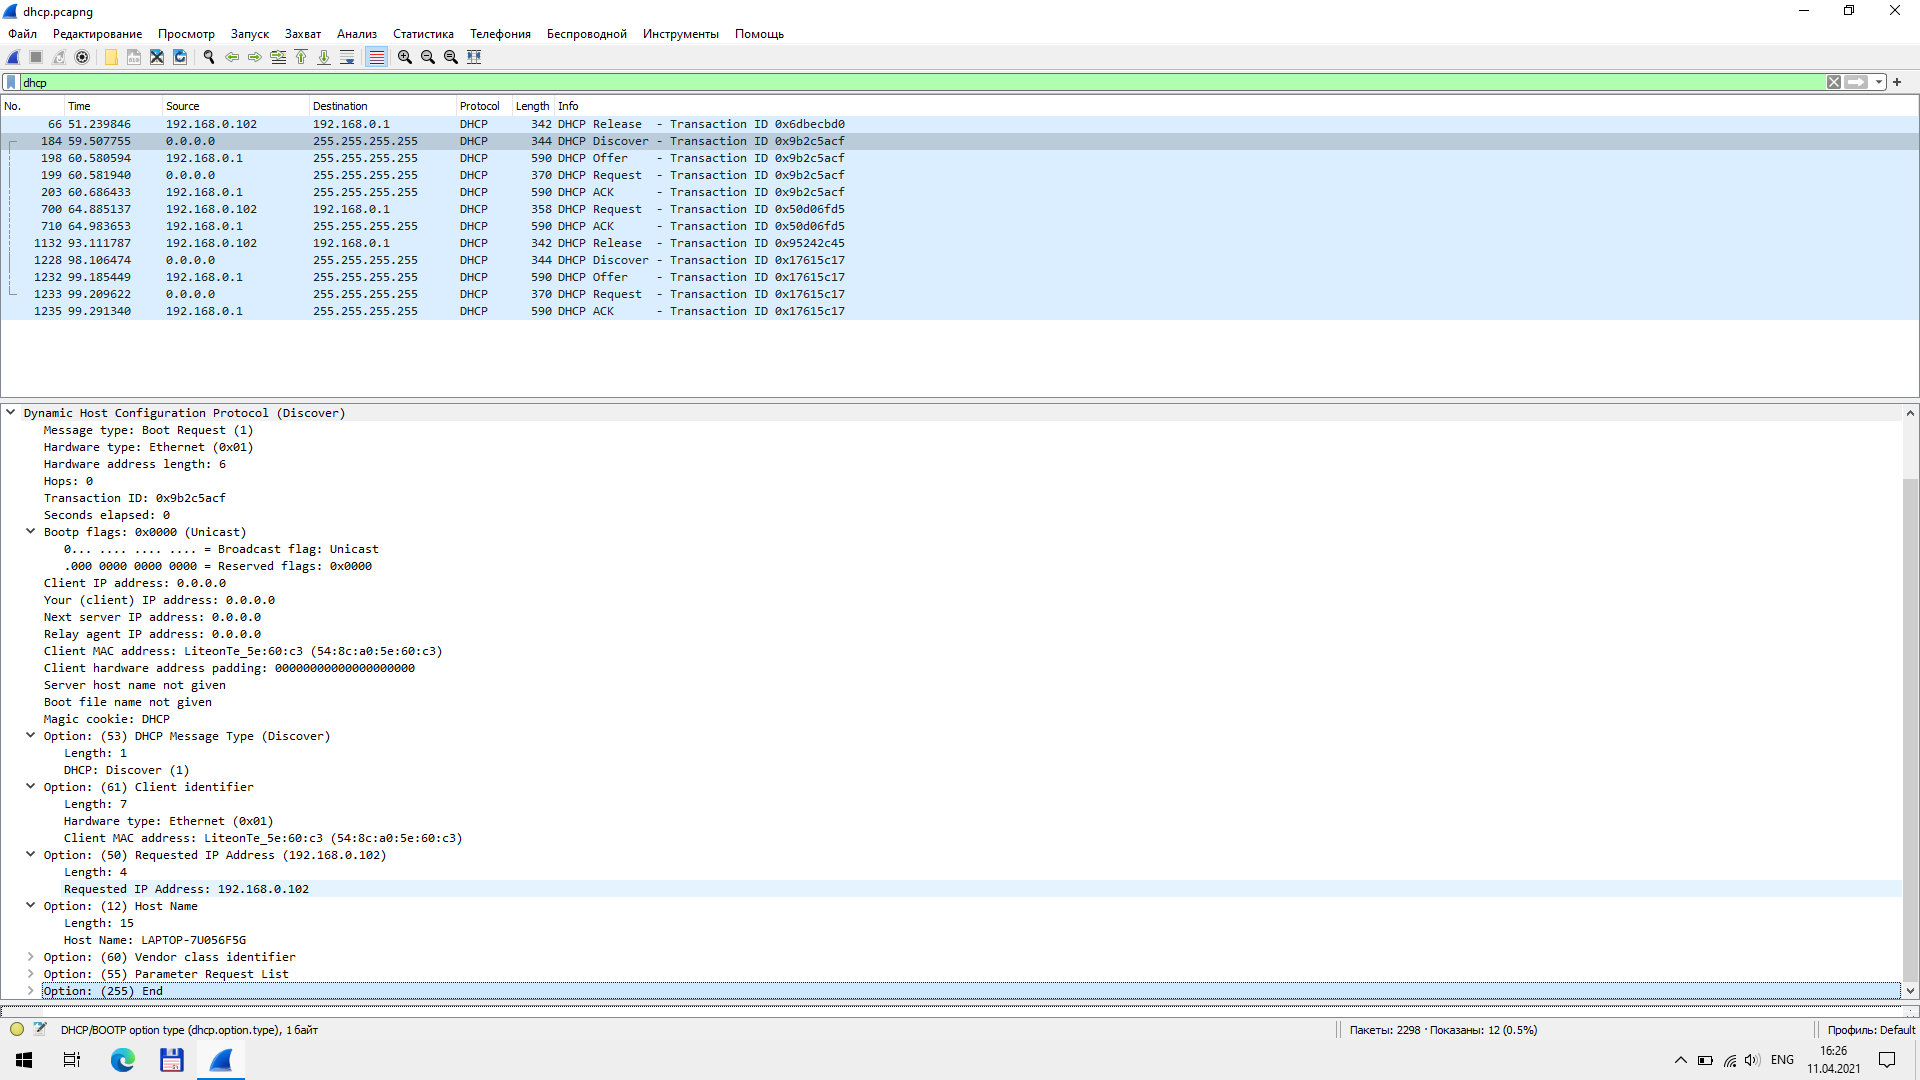
\includegraphics[width=\textwidth]{screenshots/dhcp_discover_1}

    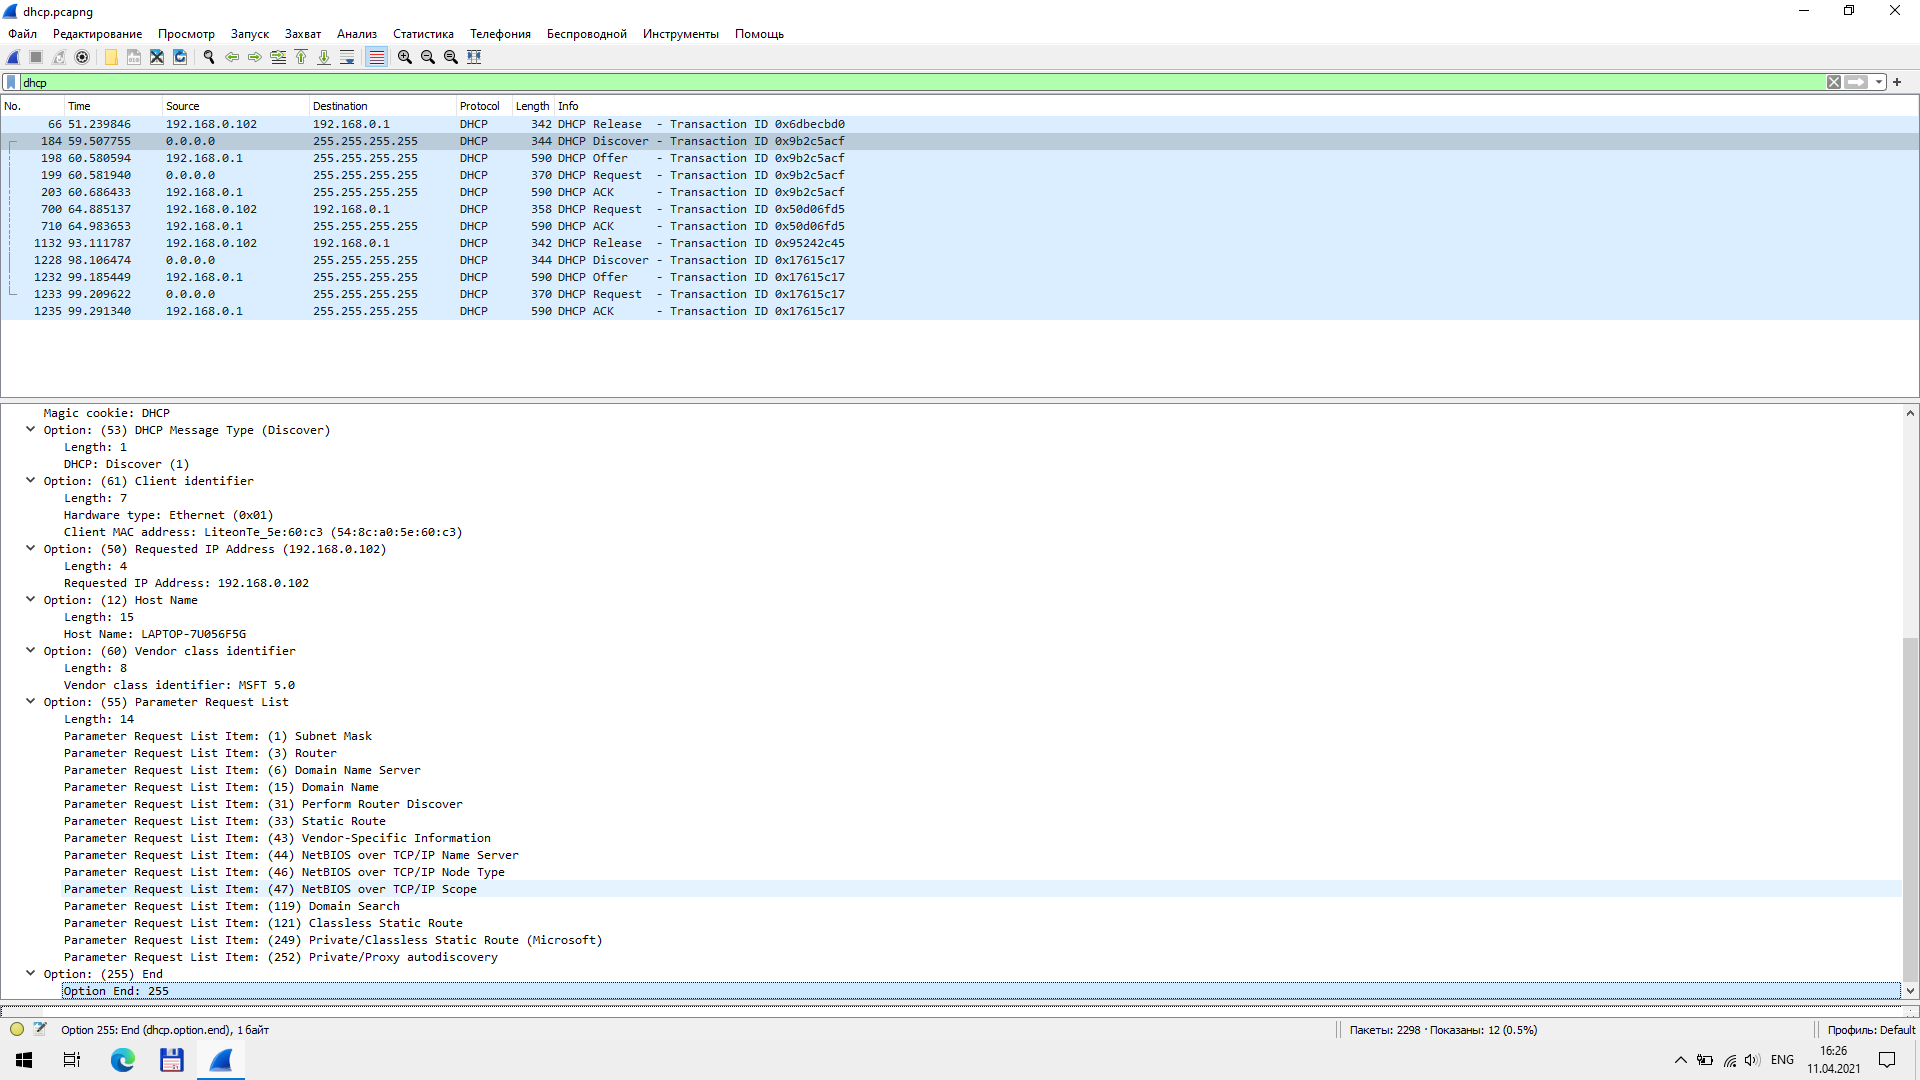
\includegraphics[width=\textwidth]{screenshots/dhcp_discover_2}

    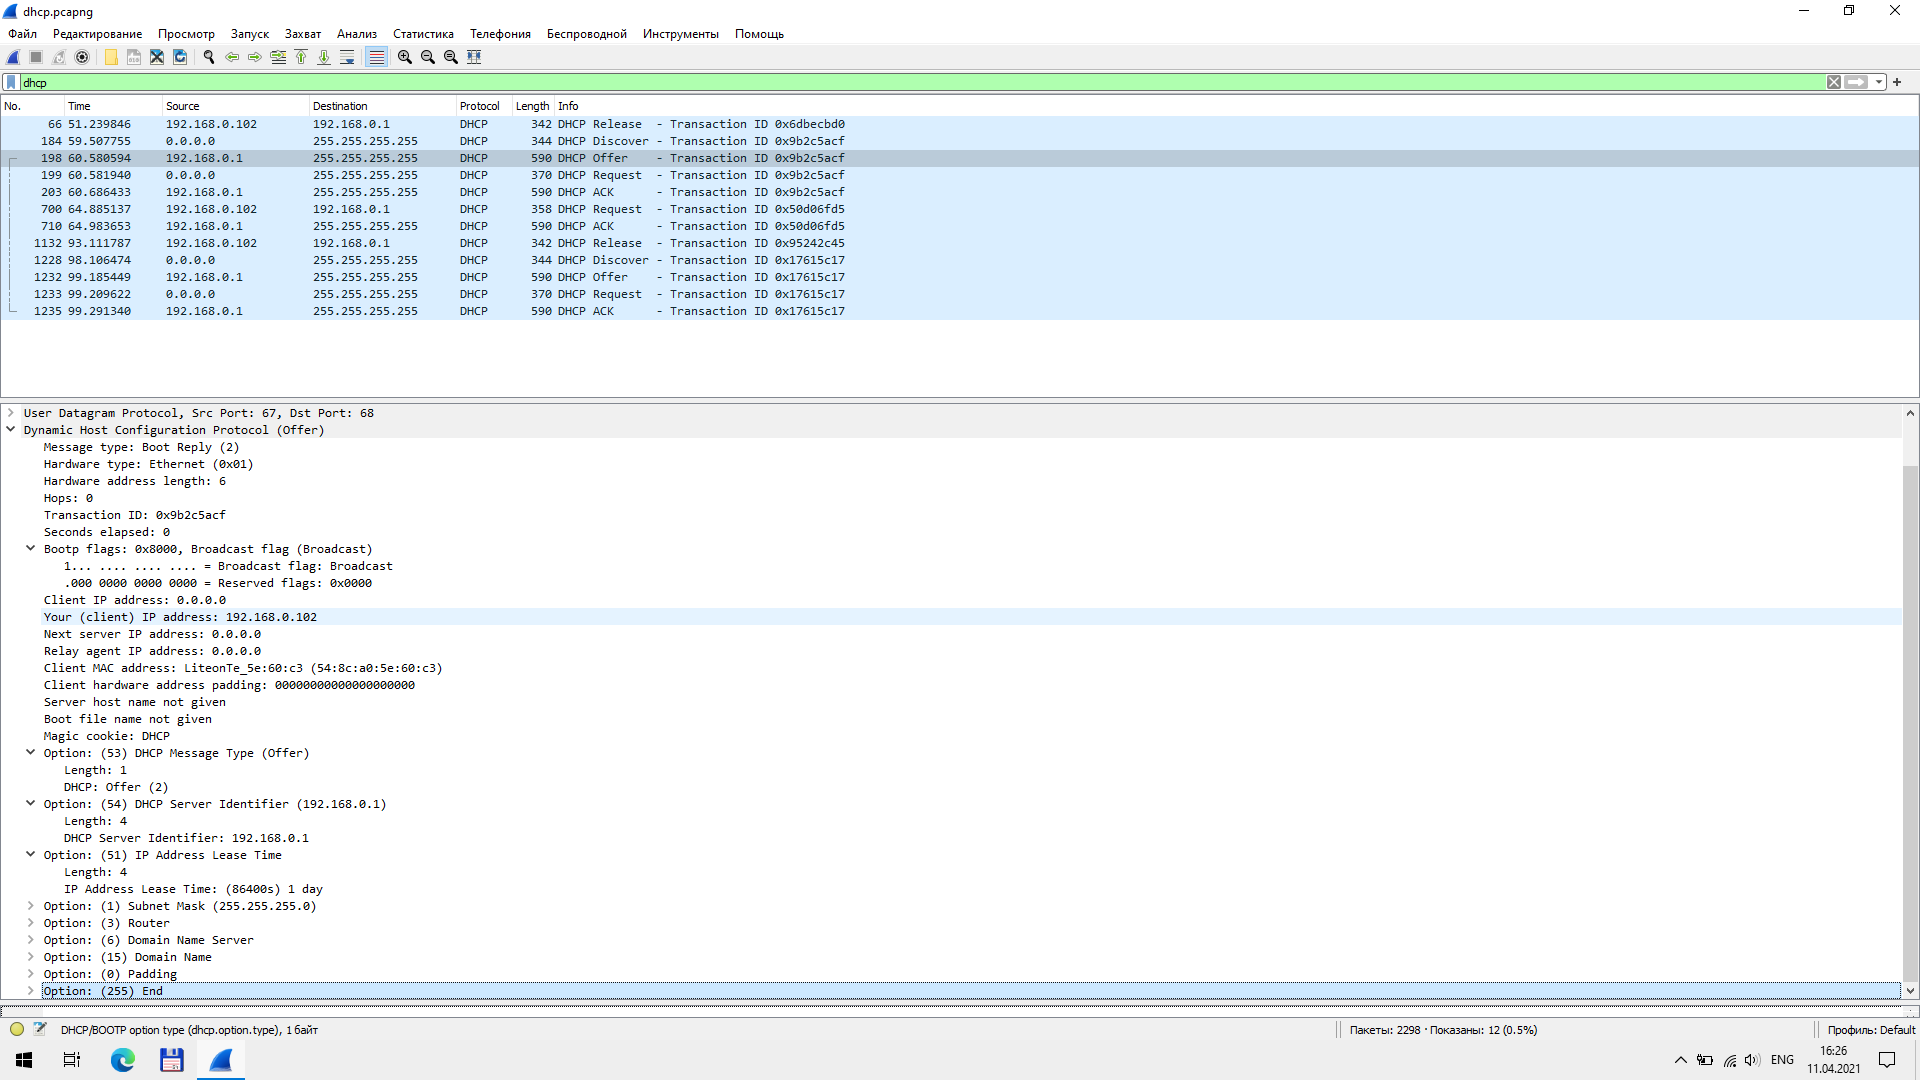
\includegraphics[width=\textwidth]{screenshots/dhcp_offer_1}

    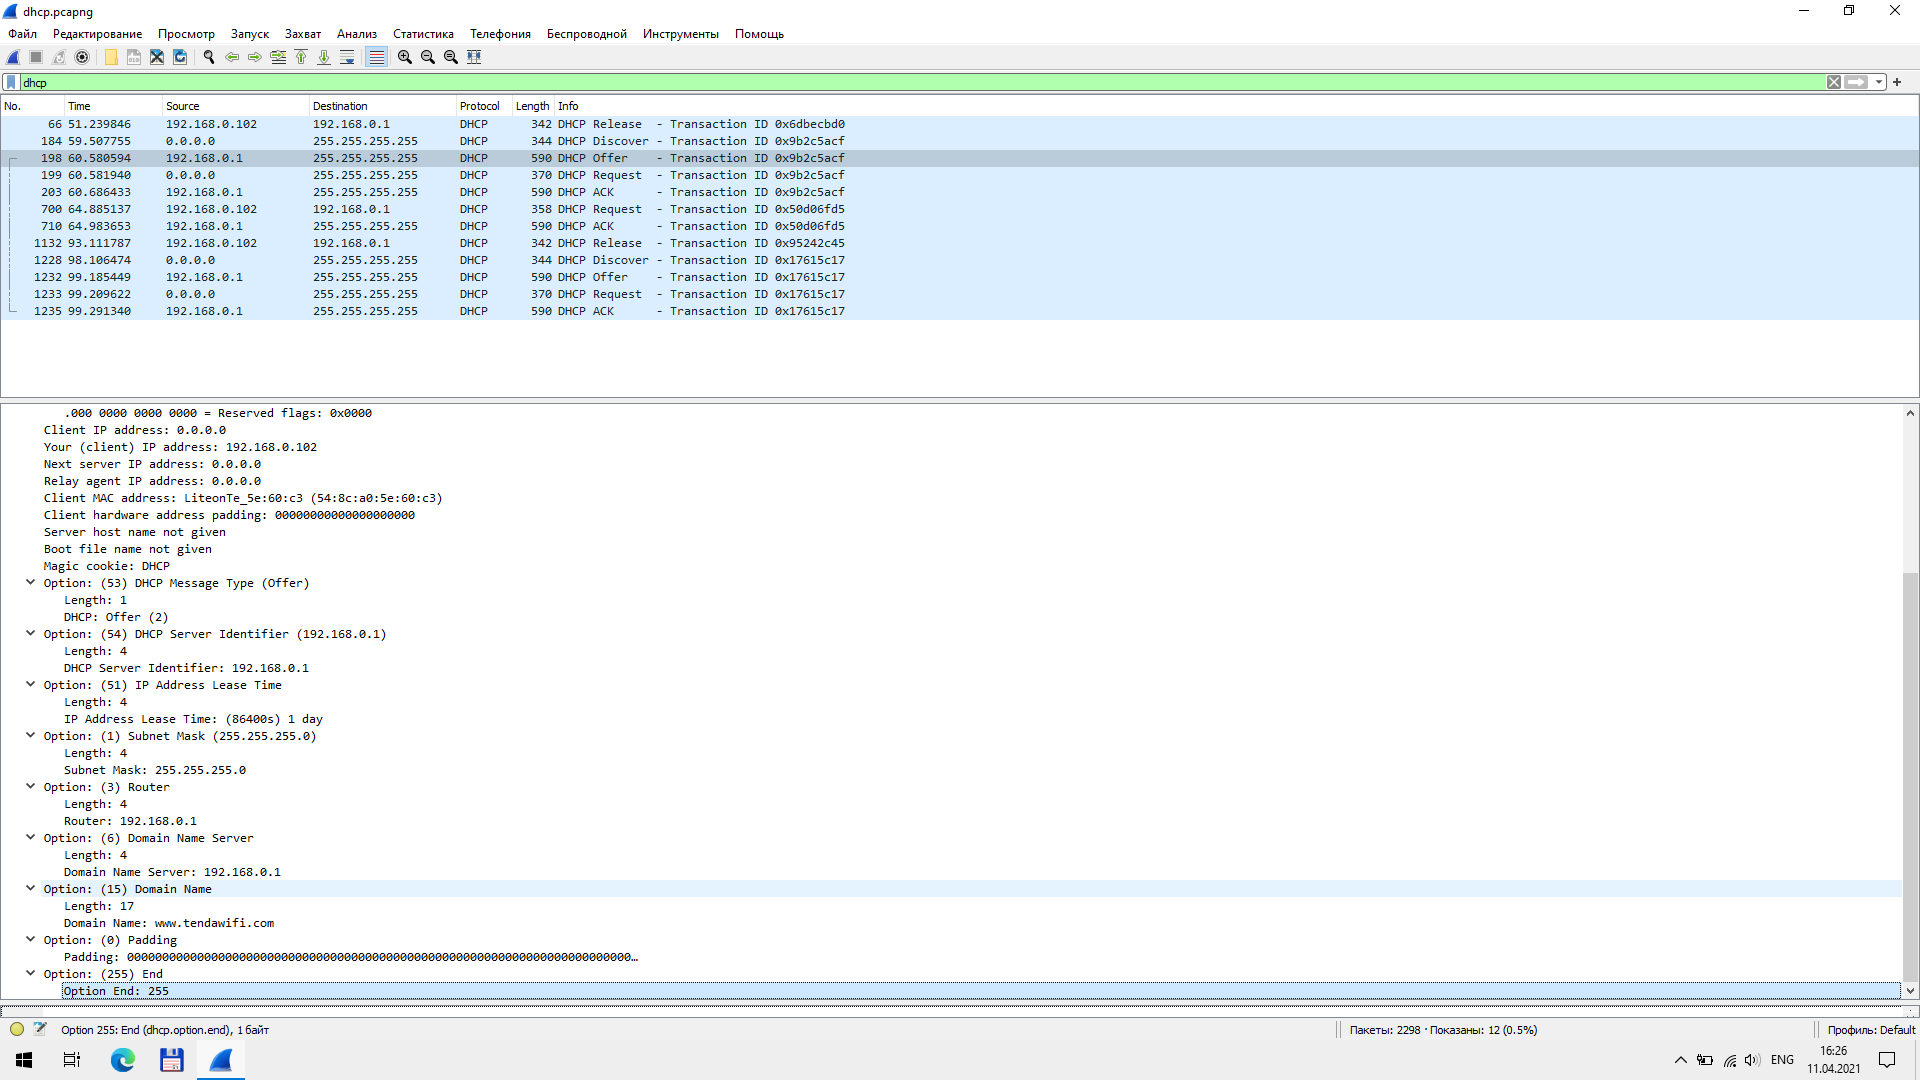
\includegraphics[width=\textwidth]{screenshots/dhcp_offer_2}

    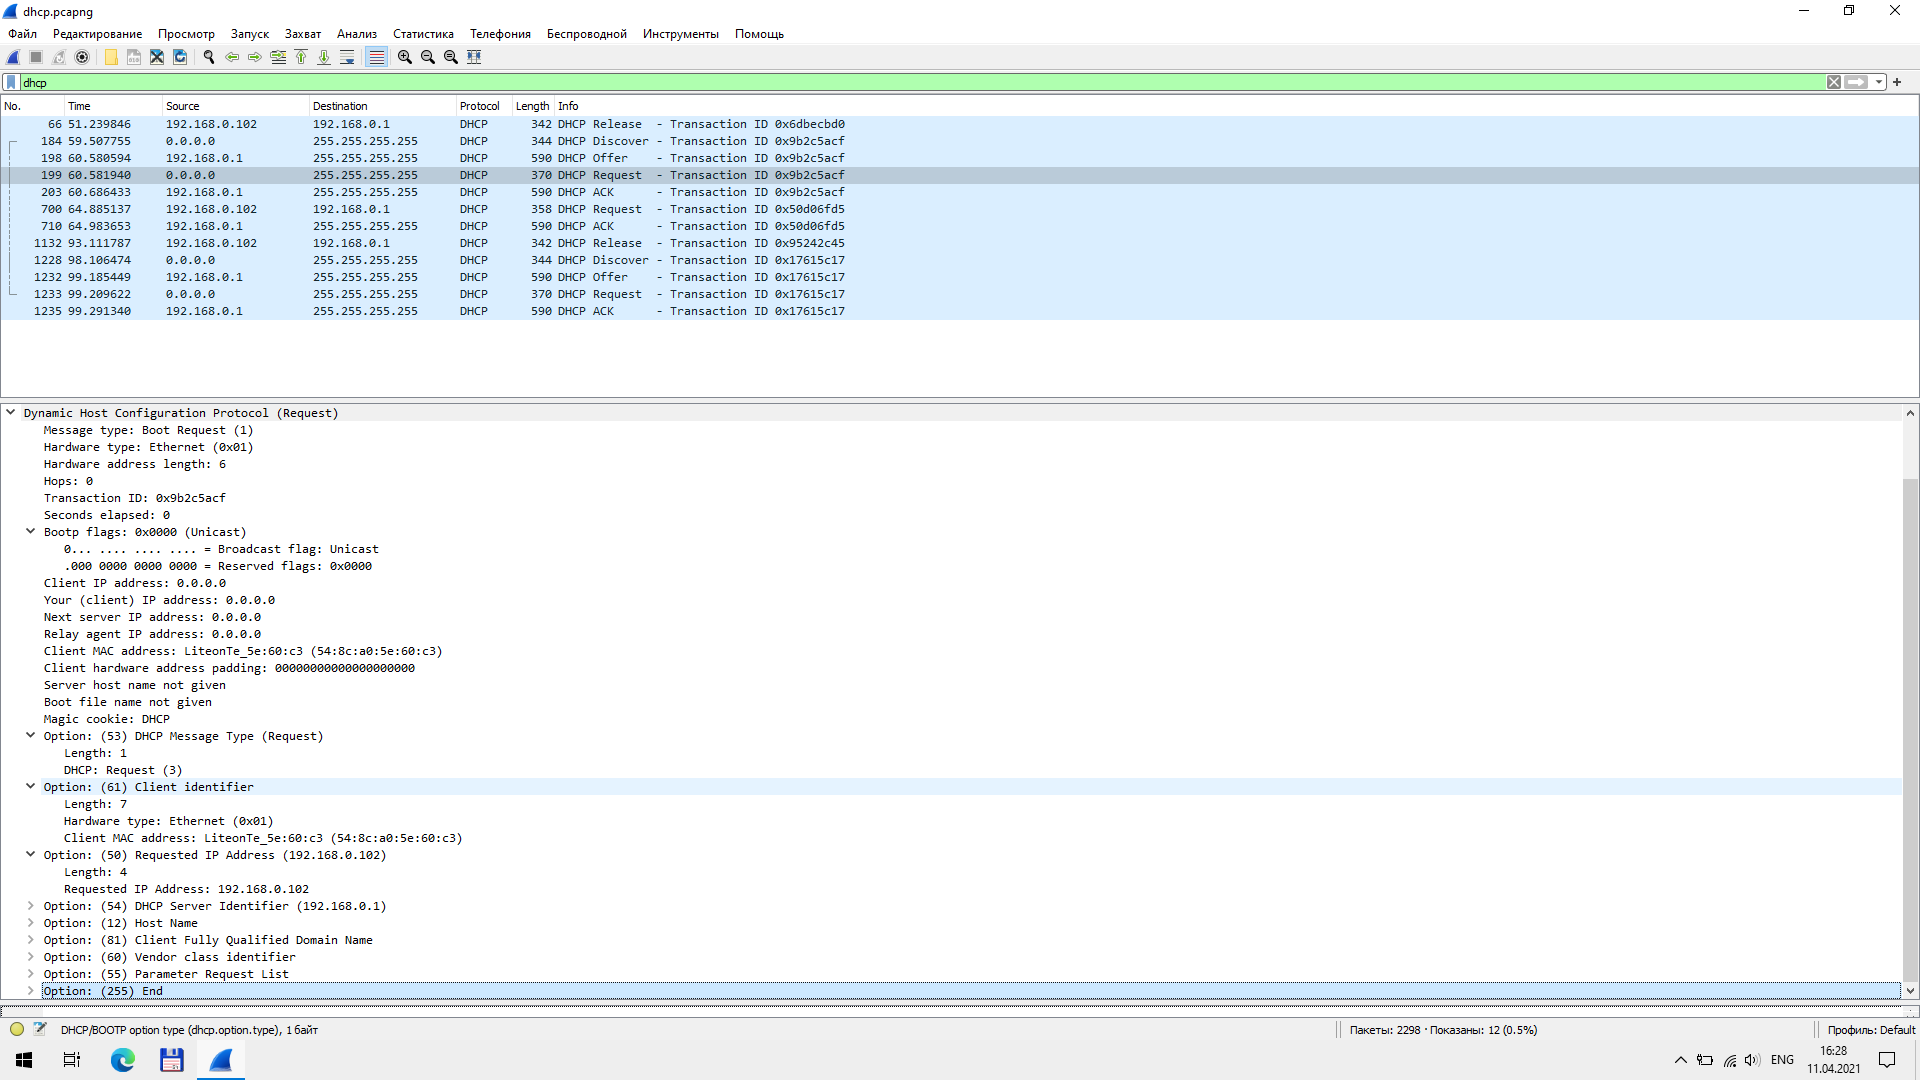
\includegraphics[width=\textwidth]{screenshots/dhcp_request1_1}

    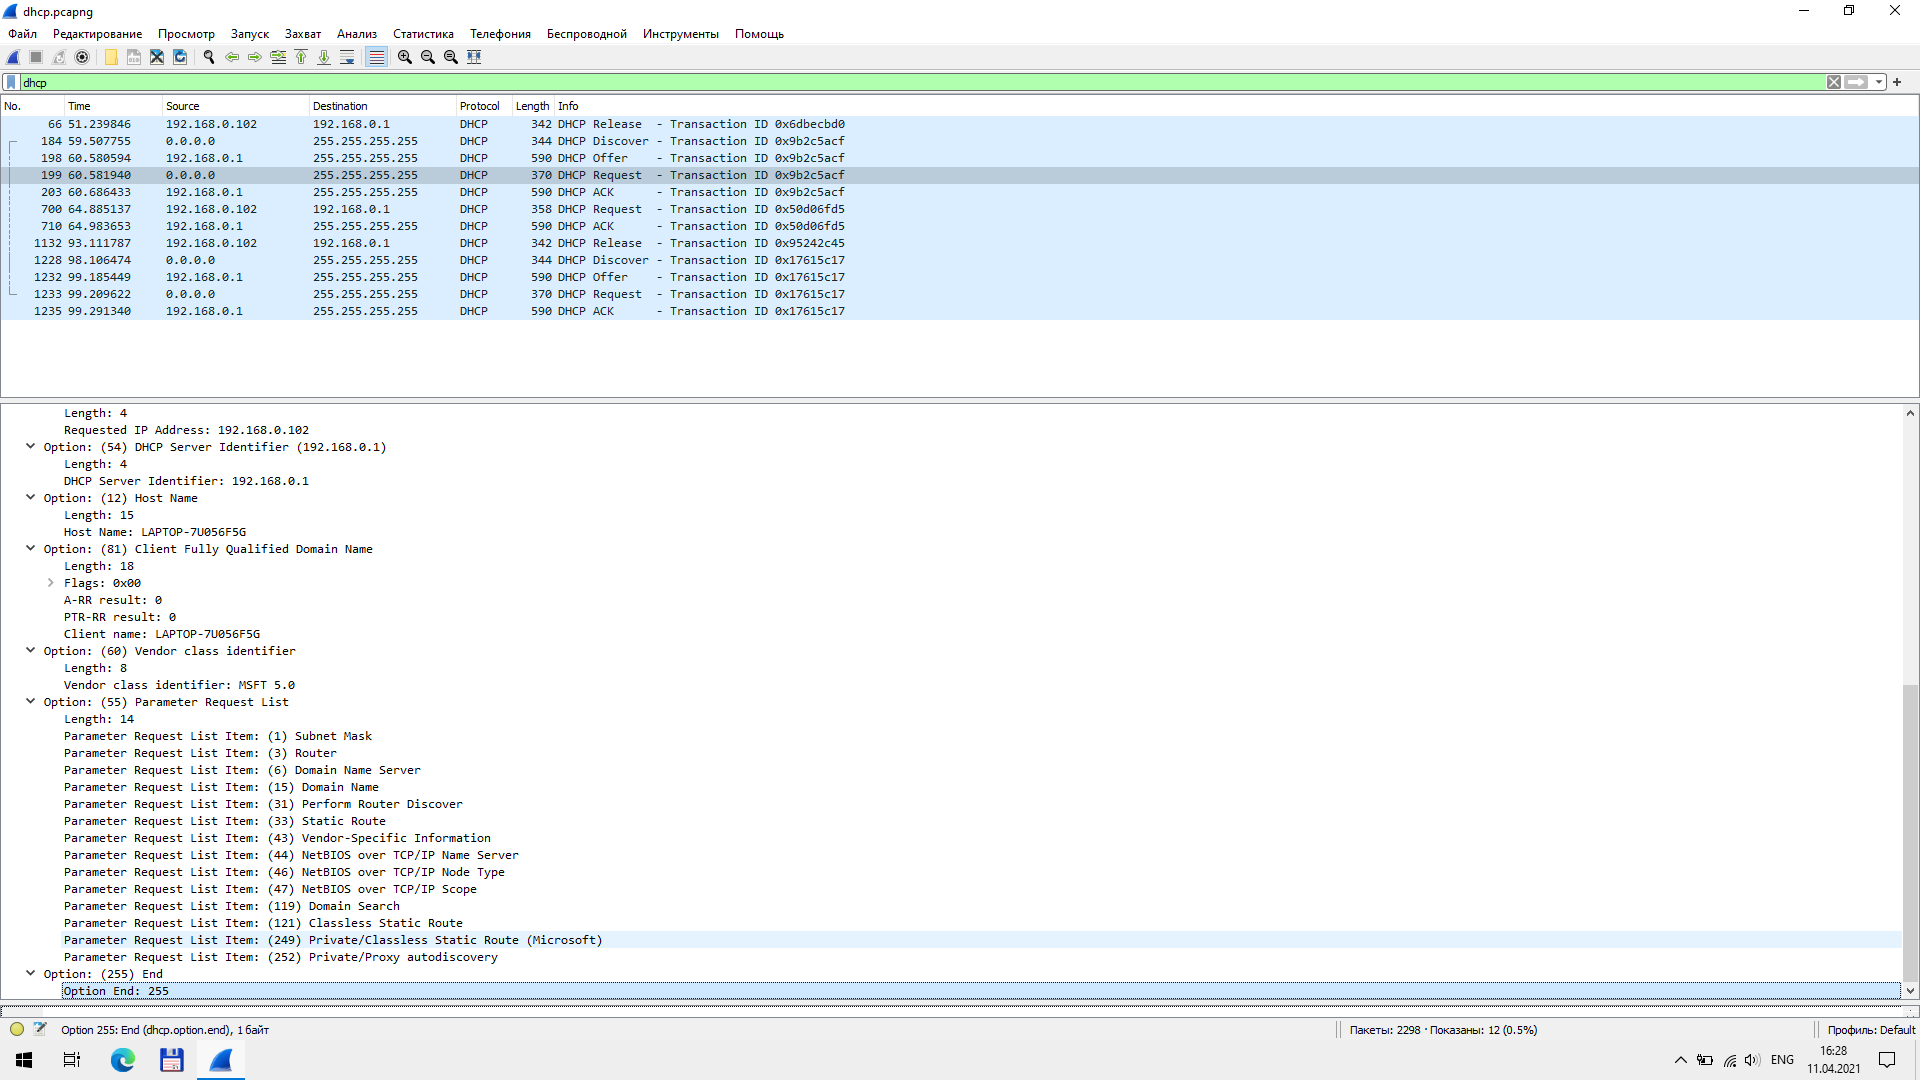
\includegraphics[width=\textwidth]{screenshots/dhcp_request1_2}

    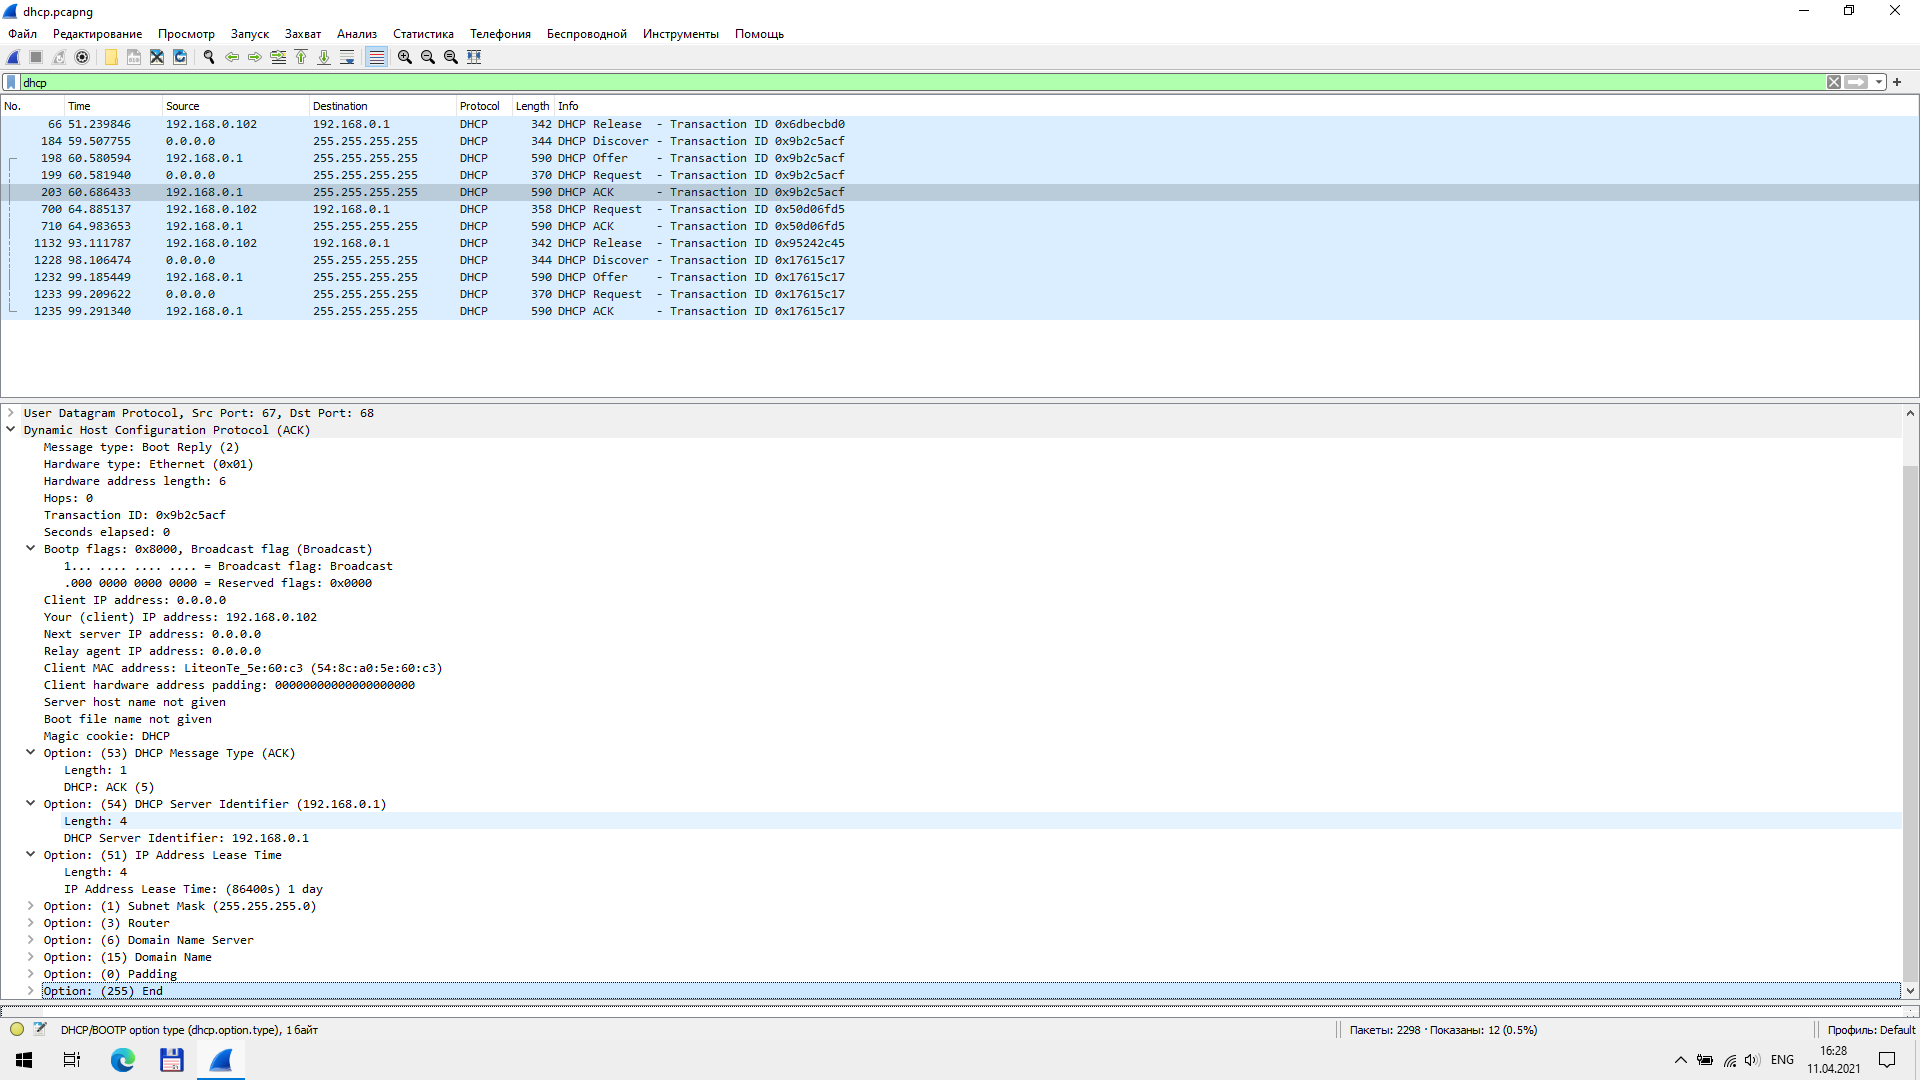
\includegraphics[width=\textwidth]{screenshots/dhcp_ack1_1}

    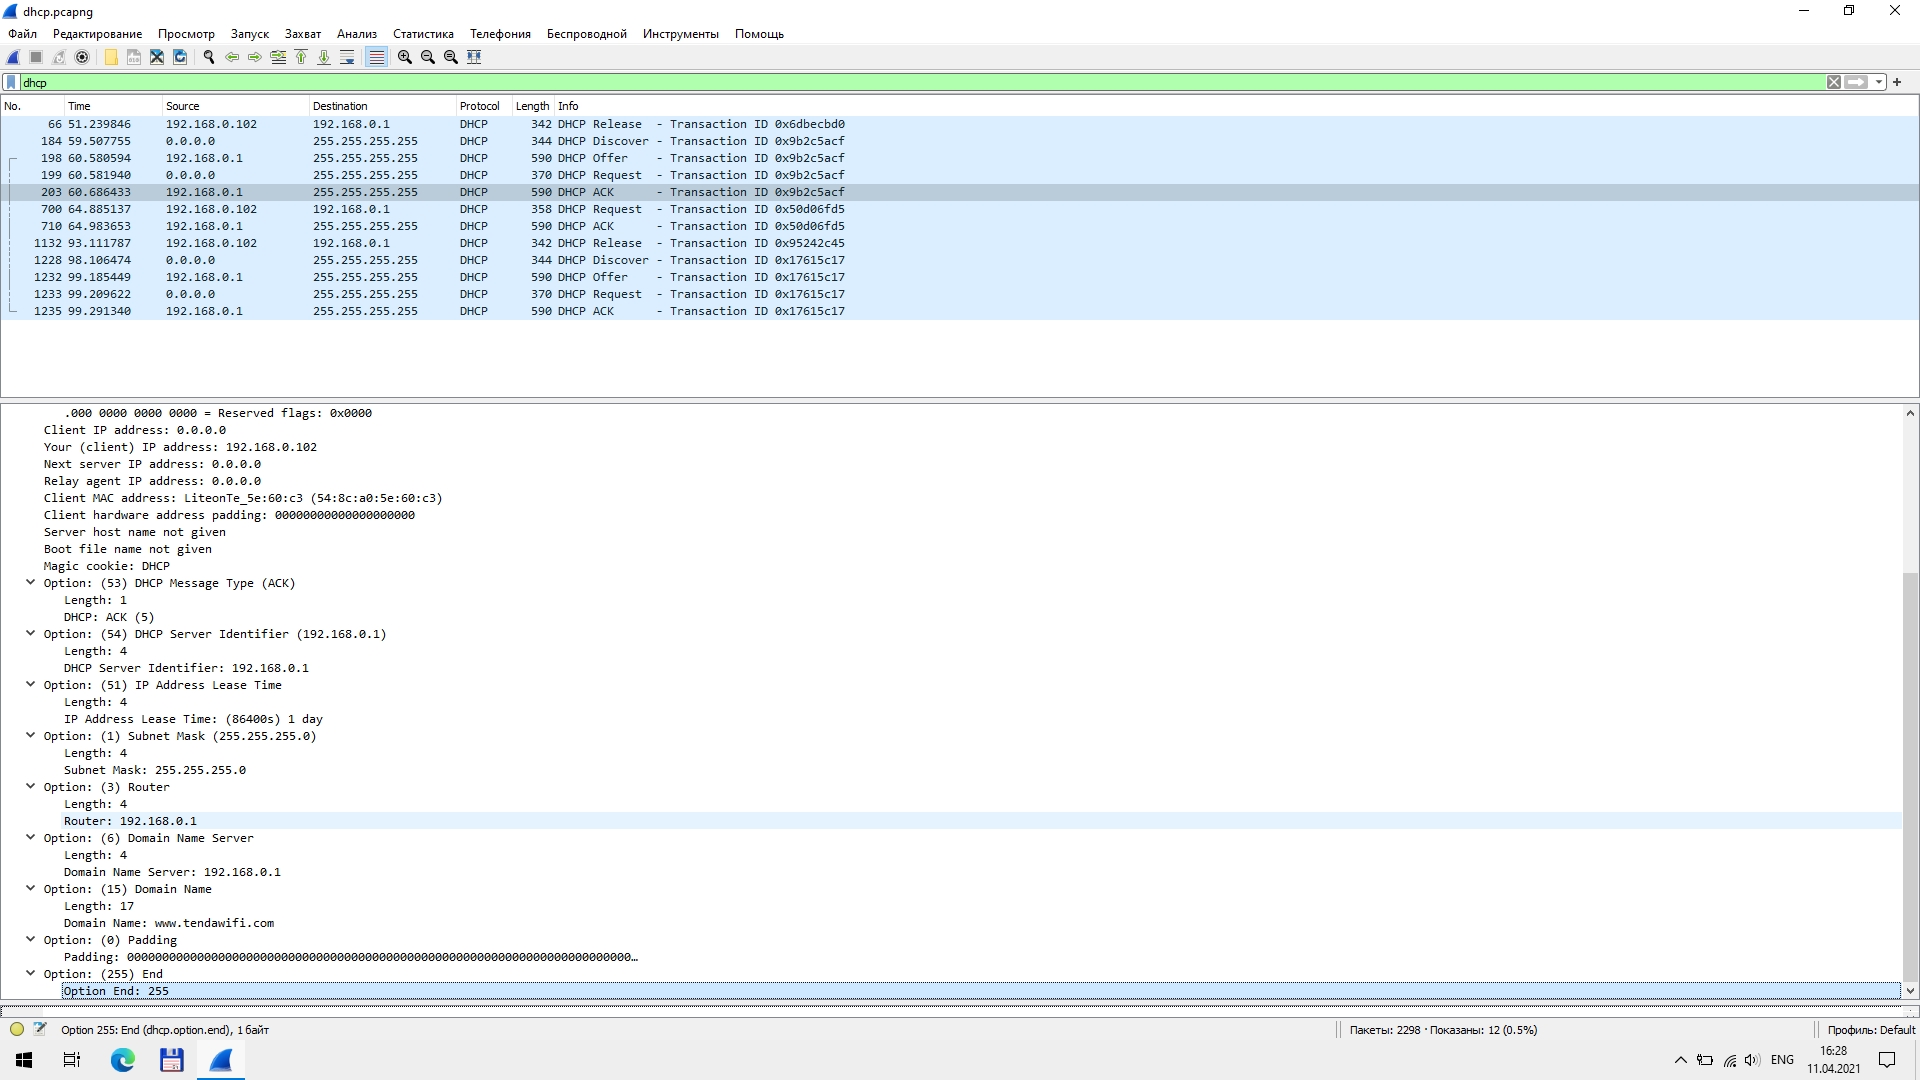
\includegraphics[width=\textwidth]{screenshots/dhcp_ack1_2}

    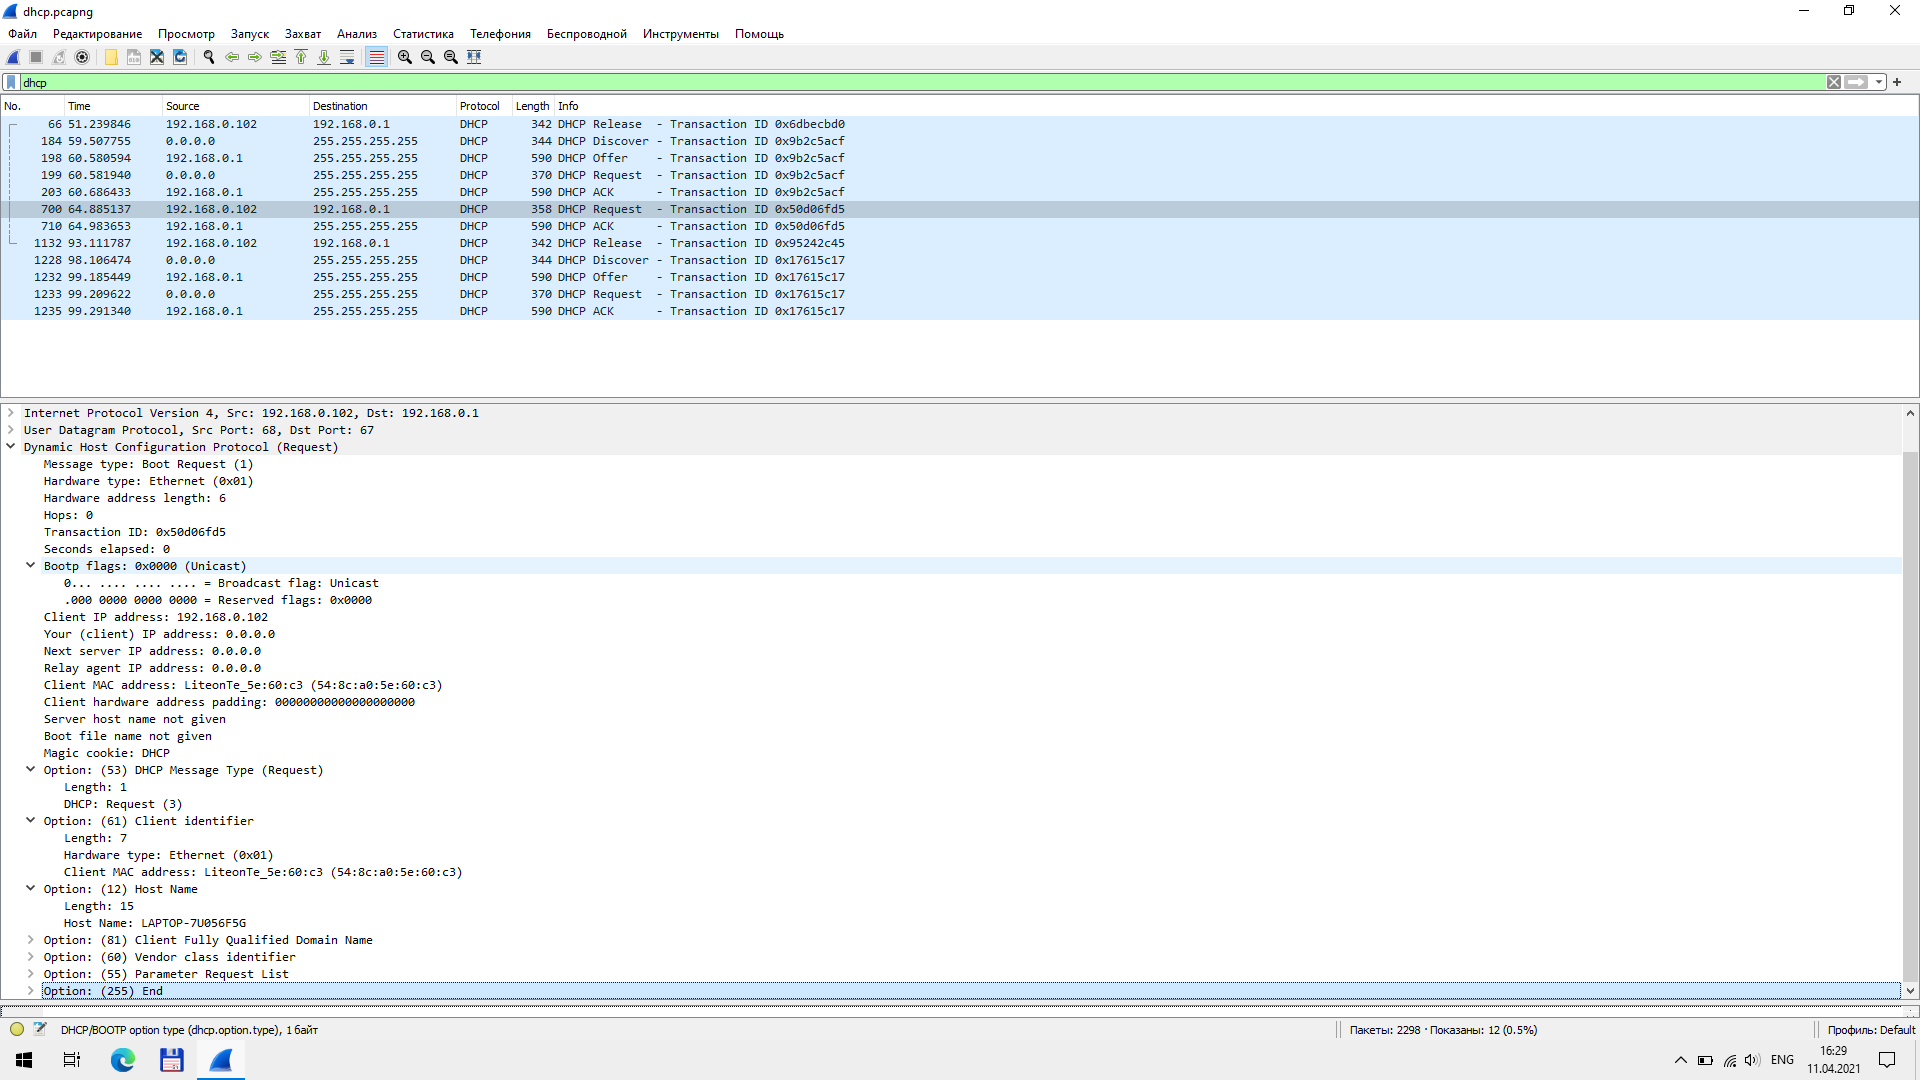
\includegraphics[width=\textwidth]{screenshots/dhcp_request2_1}

    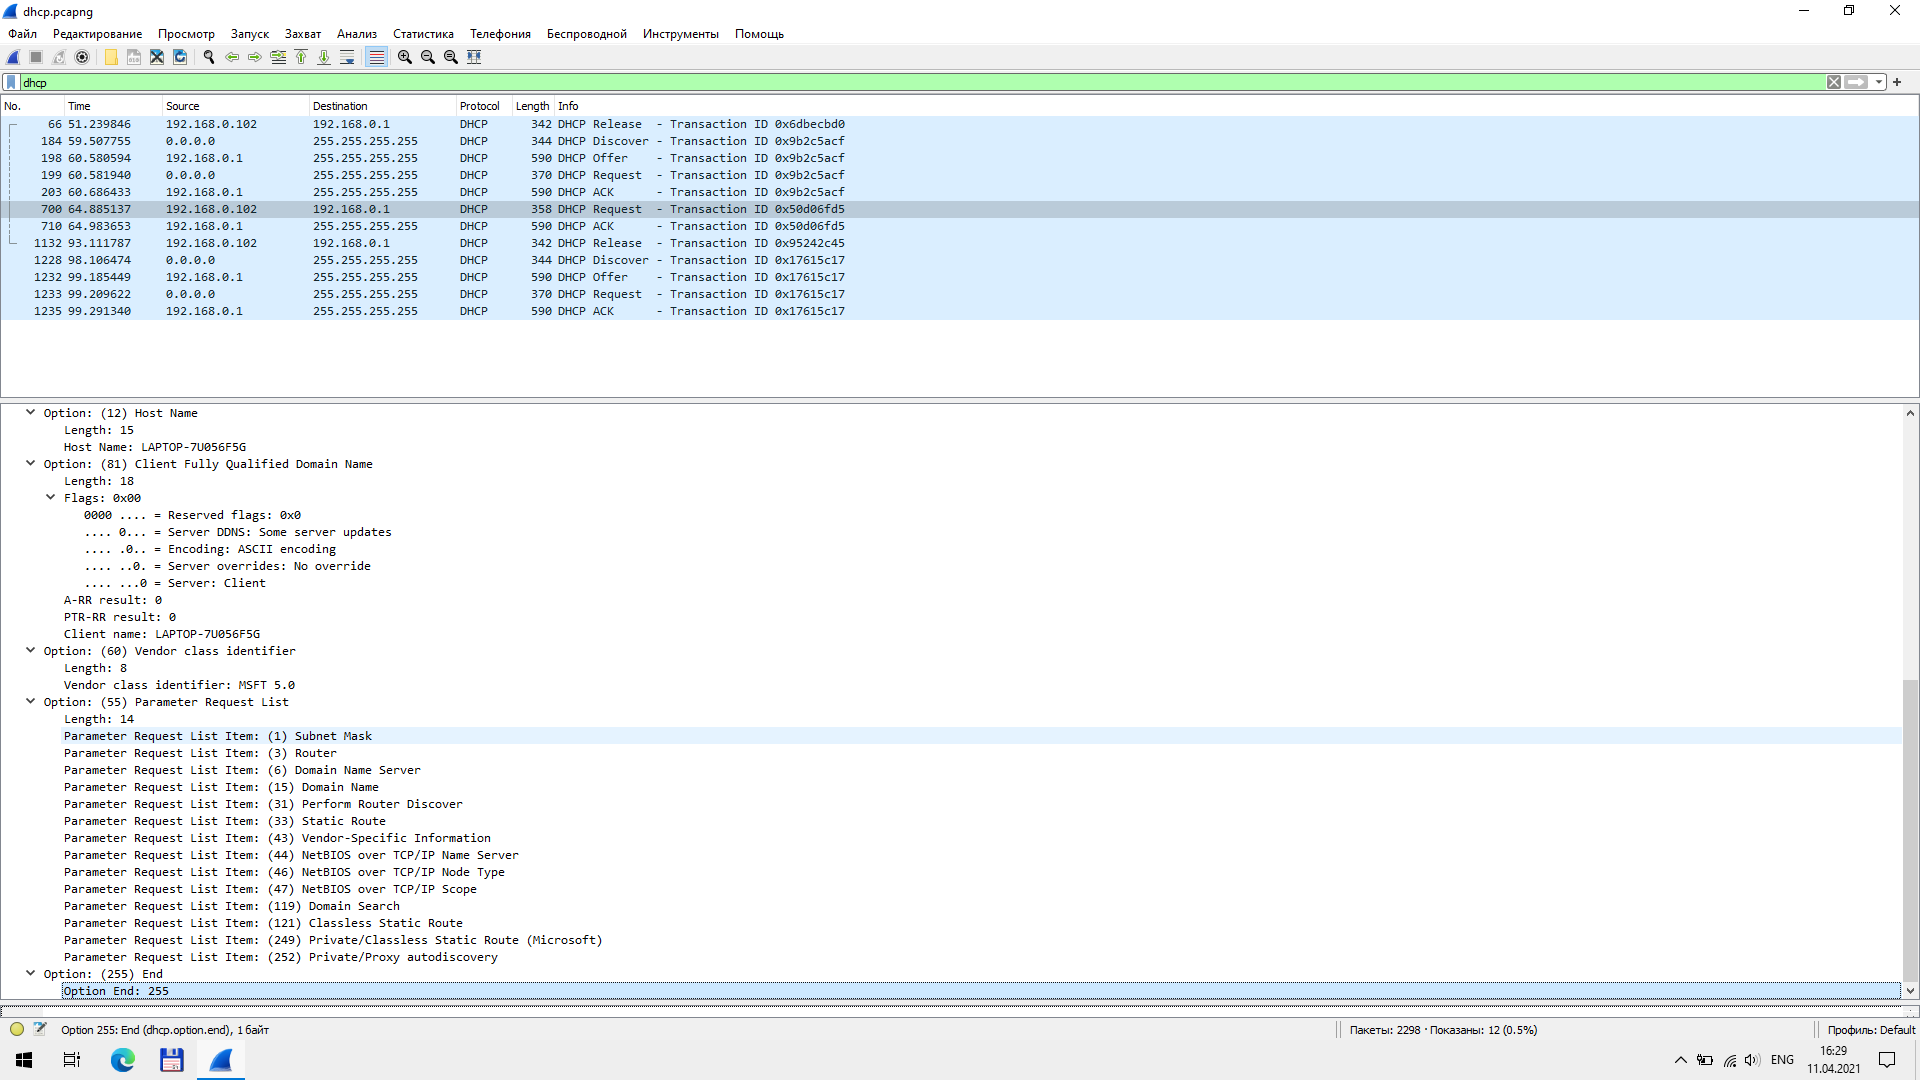
\includegraphics[width=\textwidth]{screenshots/dhcp_request2_2}

    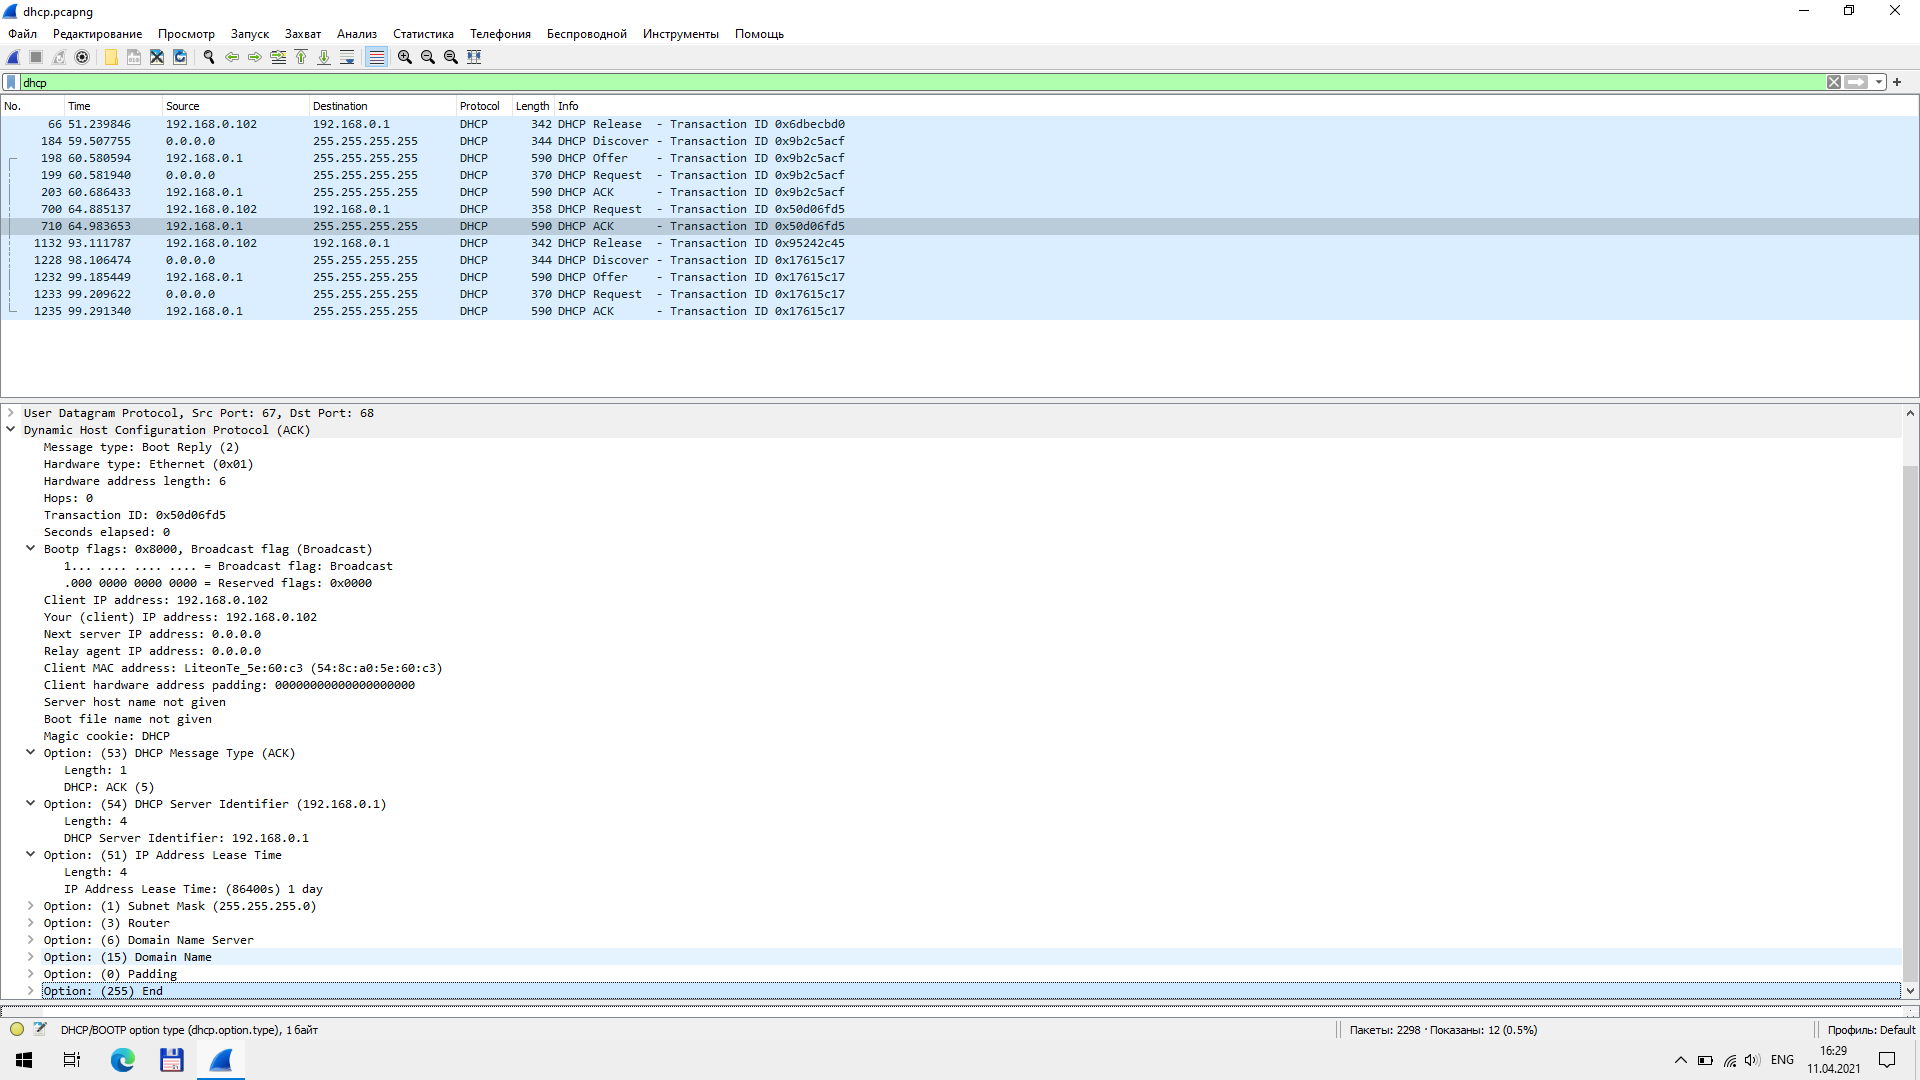
\includegraphics[width=\textwidth]{screenshots/dhcp_ack2_1}

    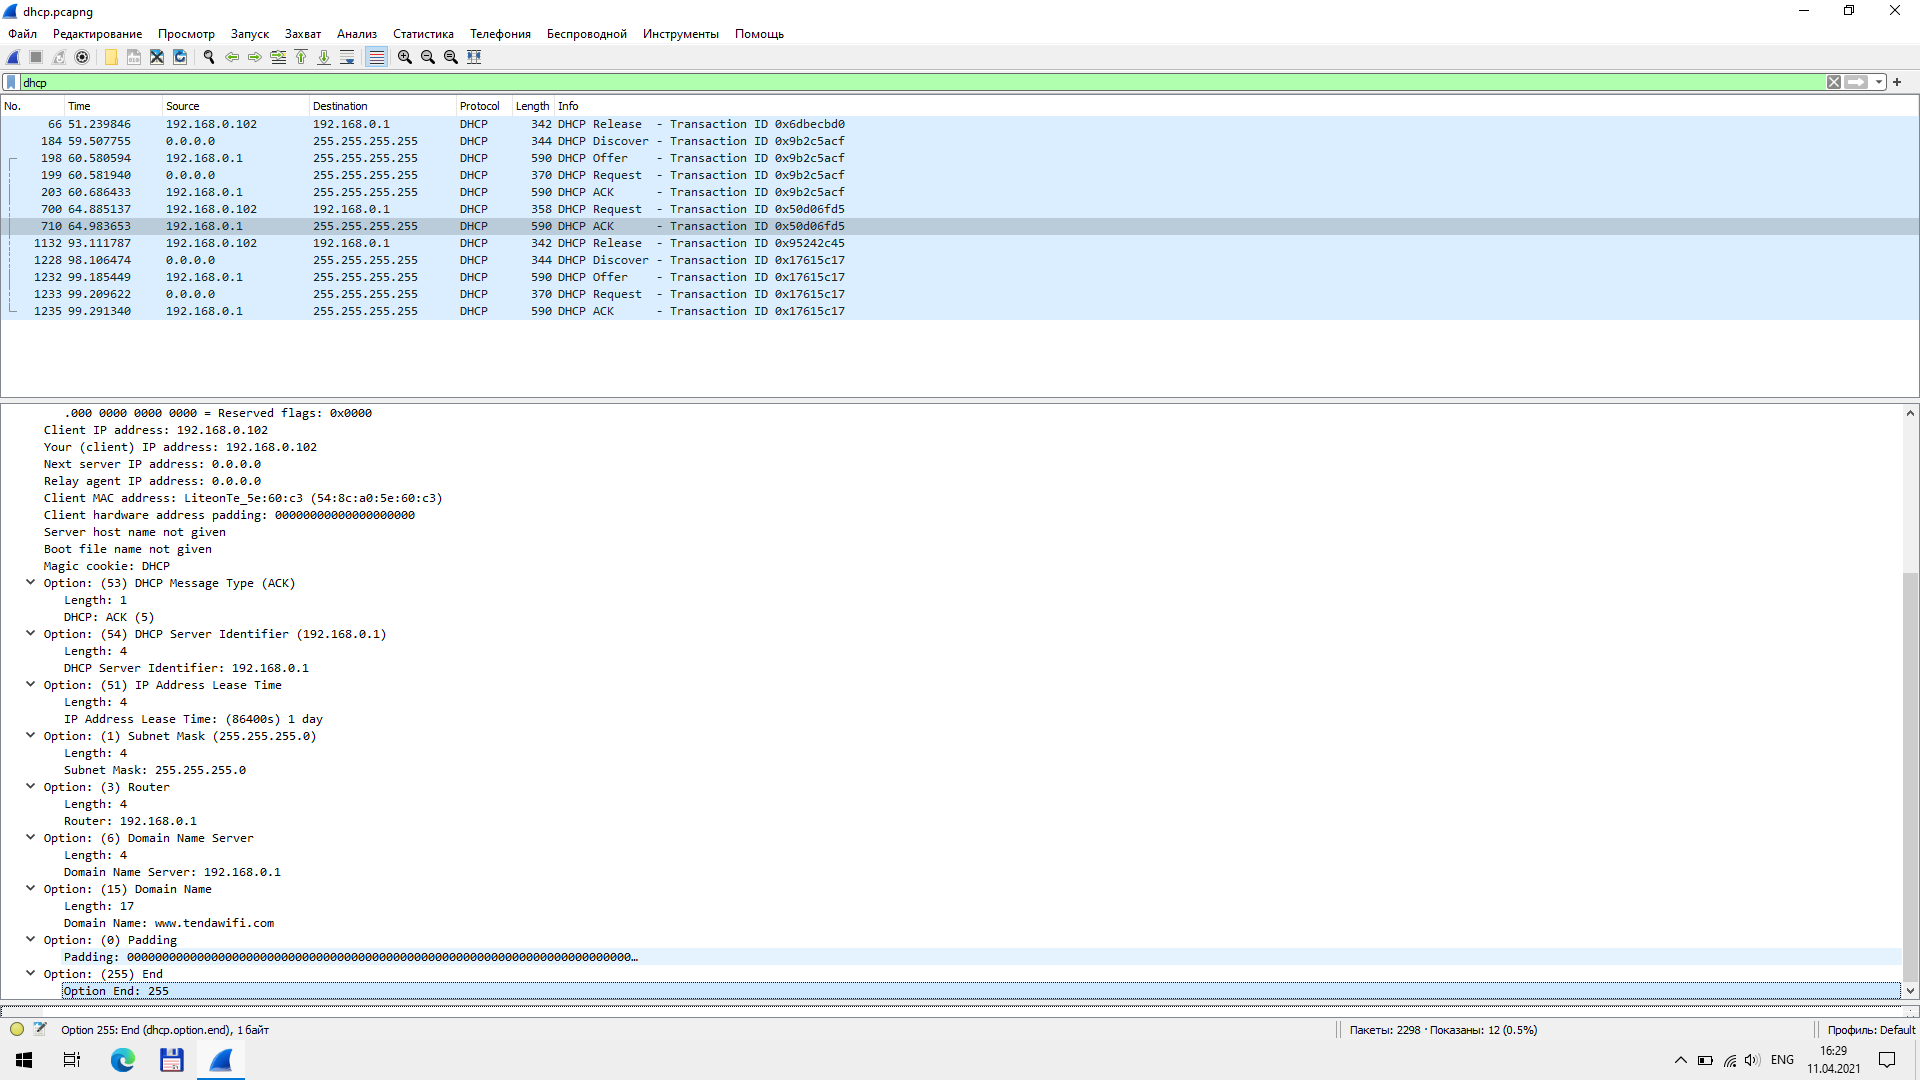
\includegraphics[width=\textwidth]{screenshots/dhcp_ack2_2}

\end{center}

\subsection{Ответы на вопросы}

\begin{enumerate}
    \item Discover \texttt{54:8c:a0:5e:60:c3} (68) $\Longrightarrow$ \texttt{ff:ff:ff:ff:ff:ff} (67)
    \item Offer    \texttt{04:95:e6:66:37:08} (67) $\Longrightarrow$ \texttt{ff:ff:ff:ff:ff:ff} (68)
    \item Request  \texttt{54:8c:a0:5e:60:c3} (68) $\Longrightarrow$ \texttt{ff:ff:ff:ff:ff:ff} (67)
    \item ACK      \texttt{04:95:e6:66:37:08} (67) $\Longrightarrow$ \texttt{ff:ff:ff:ff:ff:ff} (68)
\end{enumerate}

\subsubsection{}
DHCP Discover --- сообщение о своем существовании в сети и запрос возможных адресов,
а также сообщение последнего известного своего.
DHCP Request --- попытка занять определенный адрес на определенном DHCP сервере.

\subsubsection{}
MAC не менялись.
IP менялись, т.к. распределение IP --- и есть функция DHCP\@.
При этом менялся только IP клиента, 0.0.0.0, и в конце 192.168.0.102.

\subsubsection{}
192.168.0.1.

\subsubsection{}
Можно будет увидеть, что между DHCP Offer и DHCP Request не пришло ни одного пакета,
потому что в это время не было IP-адреса.
